\documentclass{article}

\usepackage[a4paper,margin=2.5cm]{geometry}
\usepackage{fancyhdr}
\usepackage{pdfpages}

\title{\vspace{-2cm}INFO20003 Assignment 1 - Assumptions}
\date{\today}
\author{Lucas Fern (1080613)}

\lhead{INFO20003 - Assignment 1}
\rhead{Lucas Fern (1080613)}
\pagestyle{fancy}

\begin{document}
\maketitle
In the generating the physical model the following assumptions were made:
\begin{itemize}
    \item A member must have at least one phone number.
    \item Since a full list of Titles wasn't provided, titles can be input as a string.
    \item Members can only progress through the stages of membership and cannot revert to, for example, a `Provisional fellow' if they were already a `Full fellow'. This means that the \verb|idMember| and \verb|idMembershipCategory| are a suitable composite primary key for storing a member's membership status.
    \item `Unmarried', `Married', `Widowed' and `Divorced' are the only acceptable marital statuses.
    \item The reason for rejecting an application can be stored as a string within the application and does not have to be selected from an \verb|ENUM()|.
    \item The recording of an event is stored at a URL and the URL is stored in the database.
    \item The layout options of a venue are recorded as a string and not an \verb|ENUM()|.
    \item The status of an event (`Happening Now', `Postponed', etc.) can be combined with the approval status (`Accepted' / `Rejected') to make \begin{verbatim} ENUM(`Pending Approval', `Rejected', `Upcoming', `Happening Now', `Postponed', 
      `Cancelled') \end{verbatim}
    since an `Upcoming', `Happening Now', `Postponed' or `Cancelled' event must have been approved.
    \item Postcodes cannot be stored as an \verb|int| since some countries include letters in postcodes.
    \item A 2,500 word statement can be stored in 30,000 characters and a 300 word statement in 4,500 characters.
\end{itemize}
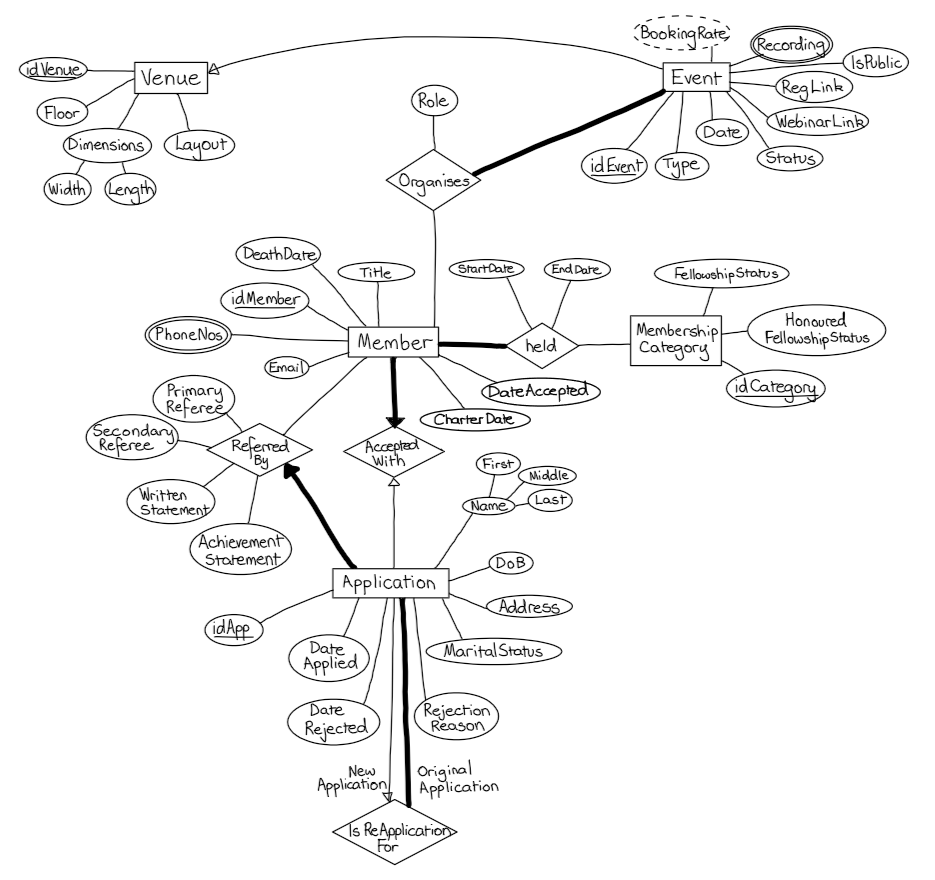
\includepdf[fitpaper=true]{logical-design.png}
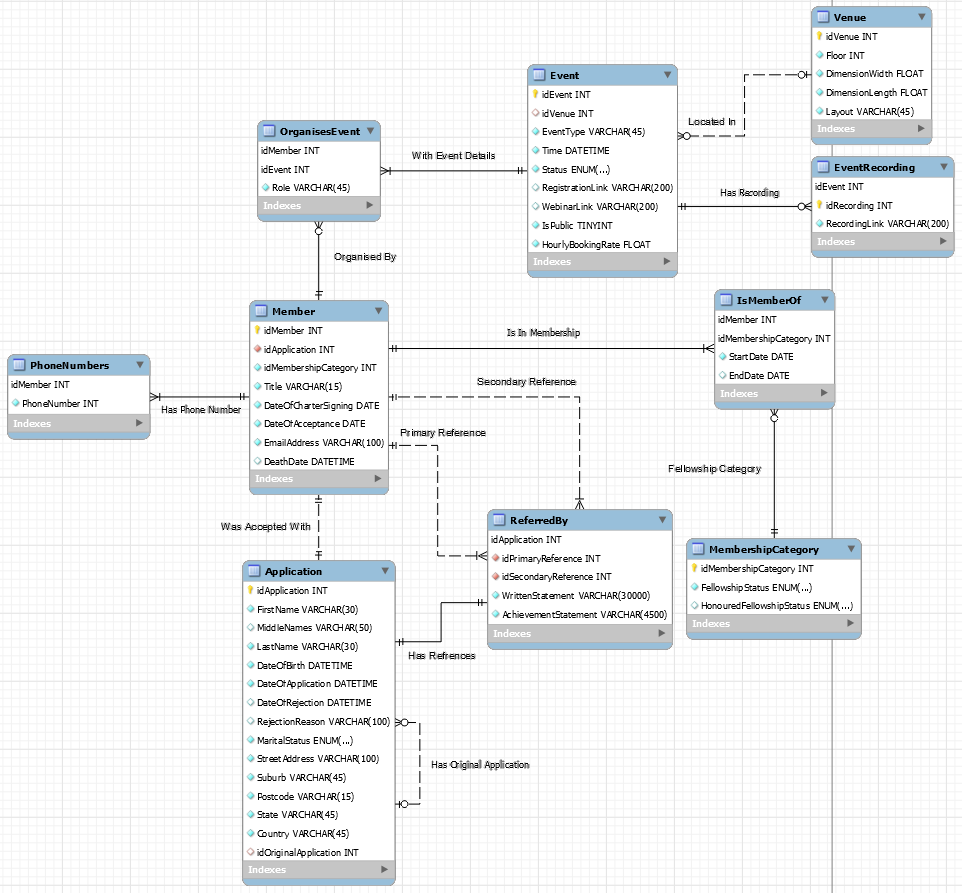
\includepdf[fitpaper=true]{physical-design.png}
\end{document}
